%!TEX root = thesis.tex

\chapter{Experiments}
\label{ch:experiments}


\section{The dataset}
A dataset was constructed where people perform the Curwen hand poses in different settings. Usually the 12 Curwen solfege hand symbols are performed in front of the torso. To increase the number of hand poses to be recognized and increase the usability, all 12 Curwen are also performed mirrored next to the body of the recorded subject, see \autoref{fig:torso}. Additionally four extra hand symbols have been added that are not part of the Curwen sequence. These last four symbols are performed next to the head. This results in a total of 28 hand poses.

\begin{figure}[tb]
  \centering
	\subfloat[in front of torso]{
		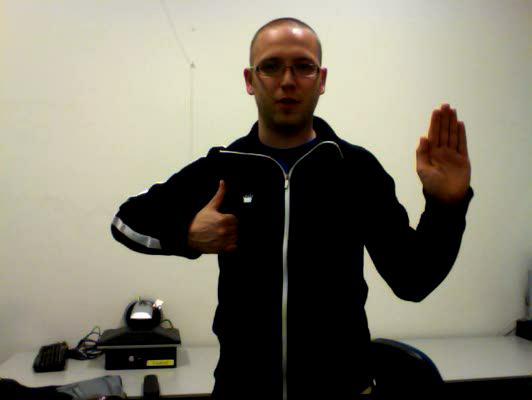
\includegraphics[width=0.4\linewidth]{figures/gijs5/13.png}
	}
\hspace{0.03\linewidth}
	\subfloat[next of torso]{
		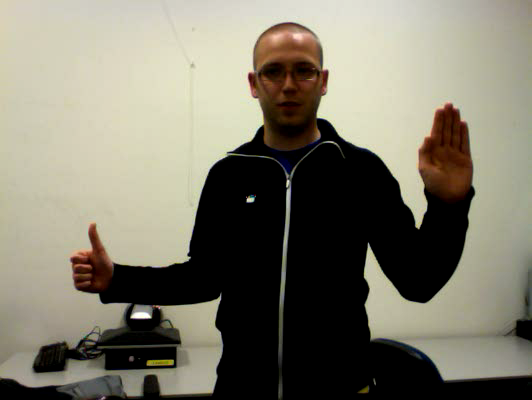
\includegraphics[width=0.4\linewidth]{figures/gijs5/1.png}
	}
  \caption{The Curwen hand poses}
  \label{fig:torso}
\end{figure}


In total there are 74 movies containing 20 different people performing the complete sequence of 28 hand symbols. At first, people were recorded performing the complete sequence 5 times, but this was taking too much time and people became impatient, after we switched to 3 movies per person. For each pose in each movie a frame was manually labeled where the person was performing the pose correctly.  The movies where recorded with  a resolution of 532x400 and a frame rate of 10 fps. The test subjects were recorded while looking at a computer screen and asked to mimic the examples as in \autoref{fig:hands}. 12 test subjects were recorded with a simple (almost empty and smooth) background (\autoref{fig:simplebackground}), 3 were recorded with a complex background (\autoref{fig:complexbackground}) and 6 were recorded with the same complex background but also with a poster with skin like colors.

The nationality of the test subjects is diverse. Half of the set is Dutch and two are from Asia. The rest is from eastern and southern Europe. 

\begin{figure}[tb]
\center{}
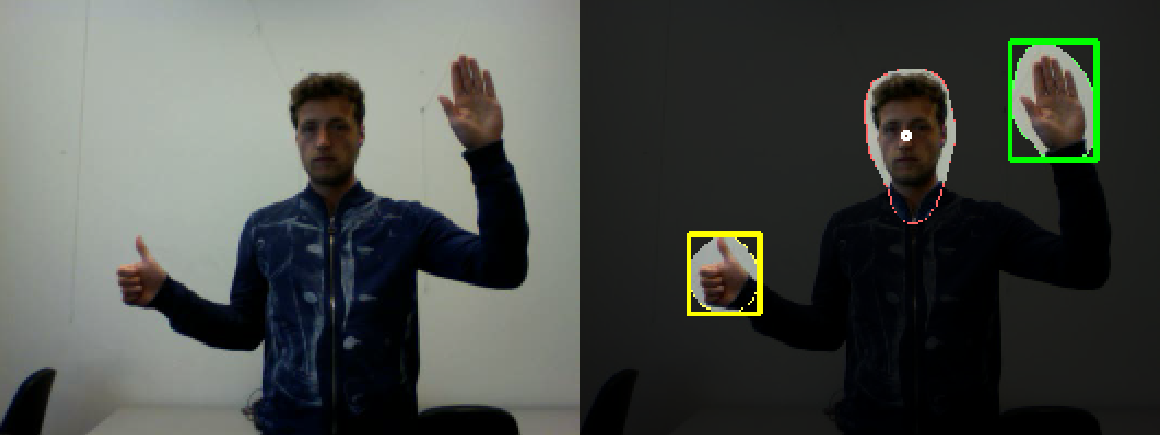
\includegraphics[width=0.8\linewidth]{figures/simple.png}
\caption{Still of movie ivo5 with simple background}
\label{fig:simplebackground}
\end{figure}

\begin{figure}[tb]
\center{}
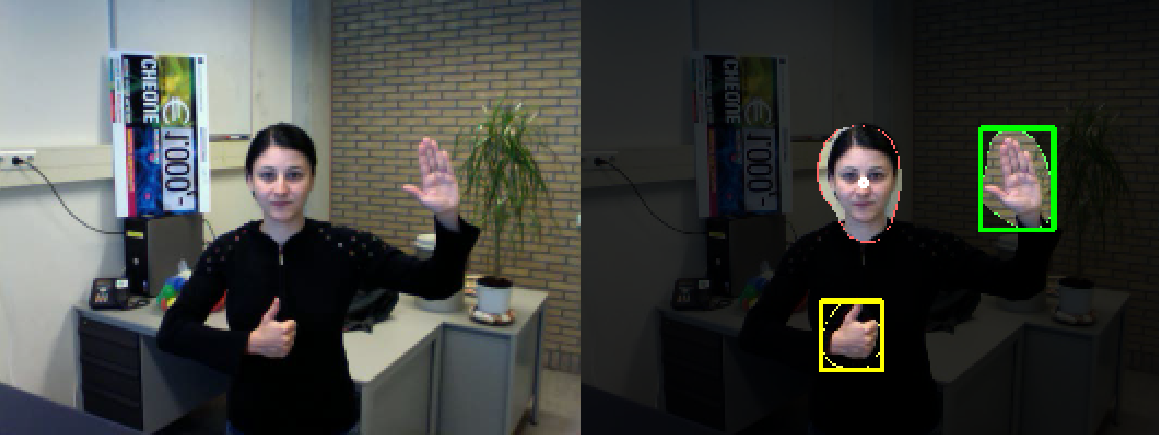
\includegraphics[width=0.8\linewidth]{figures/complex.png}
\caption{Still of movie gosia3 with complex background}
\label{fig:complexbackground}
\end{figure}

\begin{figure}[tb]
\center{}
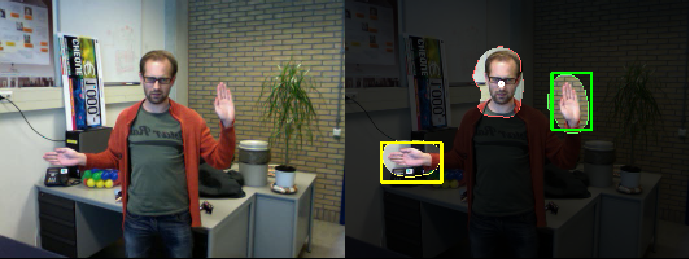
\includegraphics[width=0.8\linewidth]{figures/complexposter.png}
\caption{Still of movie sil1 with complex background with skin like poster}
\label{fig:complexposterbackground}
\end{figure}


\begin{table}
\centering
\begin{tabular}{llll}
\hline\hline
	Test Subject & Movies & Background &\\
\hline
	Anne     & 5 & Simple & \\
	Arjan    & 5 & Simple & \\
	Gijs     & 5 & Simple & \\
	Ivo      & 5 & Simple & \\
	Jasper 1 & 5 & Simple & \\
	Peter    & 5 & Simple & \\
	Hanne    & 5 & Simple & \\
	Jasper 2 & 3 & Simple & \\
	Ork      & 3 & Simple & \\
	Roberto  & 3 & Simple & \\
	Xirong   & 3 & Simple & \\
	Gosia    & 3 & Complex & \\
	Hamdi    & 3 & Complex & \\
	Michael  & 3 & Complex & \\
	Sil      & 3 & Complex + poster & \\
	Victoria & 3 & Complex + poster & \\
	Bas      & 3 & Complex + poster & \\
	Koen     & 3 & Complex + poster & \\
	Chu      & 3 & Complex + poster & \\
	Stratis  & 3 & Complex + poster & \\
\hline
\end{tabular}
\caption{Dataset details}
\end{table}

\section{Evaluation}

\subsection{Part I - Evaluating Classifiers}
In this section different classifier with different parameters are evaluated on subsets of the dataset.

\subsubsection{Method}
All hand windows for each symbol in each movie are extracted and the features are extracted and stored. This data in then imported in Matlab, where the experiments are performed. For the SVM classifier the libsvm\footnote{http://www.csie.ntu.edu.tw/~cjlin/libsvm/} package is used. To perform PCA the prtools\footnote{http://www.prtools.org/} package is used. For nearest neighbors the KNN implementation in the biolearning package of matlab itself is used. The evaluation of the classifiers is split in three runs per classifier:

\paragraph{K-fold per movie using simple dataset only}
Only the movies with a simple background are used. For each run one movie is used for testing and all other movies are used for training. For each recorded person in the test set there are also 2 or 4 recordings of him or her used in the train set. This setting mimics the real life situation where the system is pre-trained with other people \emph{and} the user, with a simple background.

\paragraph{K-fold per person}
All movies or used, but per person the movies are used for testing and all other movies for training. Both complex and simple backgrounds are used. This setting mimics the real life situation where the system is pre-trained with only other people than the user of the system, and the background is not necessarily simple. 

\paragraph{Simple as train set, complex as test set}
The classifier is trained with all movies with the simple background, and as a test set the movies with the complex background are used. This mimics the real life situation where the training is with recordings in optimal conditions, but the system is used in a complex environment like a living room. Also the system is not trained by the user.


\subsubsection{Test setting}
For the number of neighbors for $k$-NN a small number of tests where run, and a value between 3 and 10 for N yielded similar performance. Since a lower number of $k$ can give better performance $k=3$ was used for all experiments.

When PCA was performed on the dataset the smallest eigenvectors where removed so 95\% of the original variance was remaining. On the simple dataset reduce the dimensions from 3780 to 594 dimensions. For the complex set combined with the simple set the dimensionality is reduced to 688 dimensions, for complex only 283 and for the complete dataset 749.

For SVM two kernels are evaluated, RBF and $\chi^2$. The $c$ for both kernels and $\gamma$ for RBF values where found by an extensive grid search on the `per person' test set with only the simple movies performed on a small cluster in the ranges $2^{-3}$ to $2^{15}$ for $c$ and $2^{-15}$ and $2^3$ for $\gamma$. The most optimal values for $\gamma$ is 0.03125. With this $\gamma$ changing the value for $c$ didn't have much effect on the performance, so a value of 64 was taken.

For calculating the HOG features the same parameters as \citep{watanabe2009} are used, except that the image is not resized to 64 by 128 pixels, but 128 by 128 pixels.

To be able to compare the HOG and SURF, the SURF descriptor is configured to work with a fixed set of interest points set up as a dense grid - the same set used for HOG. This results in a 13440 dimensional feature vector. Also using the interest point detection is a expensive operation, calculating this on a small image takes about 500 ms which makes it unusable for real-time operation.

The Curwen hand symbols that are closely related in a musical scale way are quite similar, for example \emph{Re} and \emph{Ri} (\autoref{fig:reri}). It is expected that a lot of misclassifications will be caused by this similarity. To investigate the impact, 2 different scores are calculated, one for the major scale and one for the full scale. The full scale threats every class as a single class, for the major scale the notes in the major scale and their corresponding similar notes are joined into one class. \emph{Do} is combined with \emph{Di}, \emph{Re} with \emph{Ri}, \emph{Fa} with \emph{Fi}, \emph{Sol} with \emph{Si} and \emph{La} with \emph{Li}.


\begin{figure}[tb]
  \centering
\subfloat[Re]{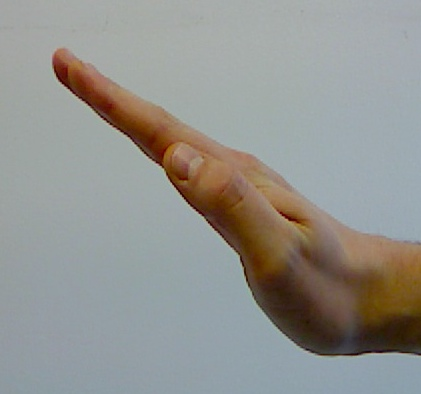
\includegraphics[width=0.2\linewidth,height=0.15\linewidth]{figures/examples/2.jpg}}
\hspace{0.03\linewidth}
\subfloat[Ri]{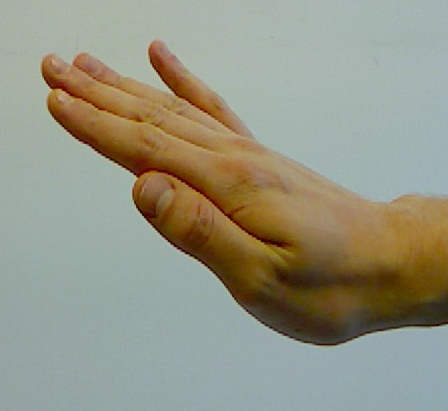
\includegraphics[width=0.2\linewidth,height=0.15\linewidth]{figures/examples/3.jpg}}
  \caption{Hand poses for \emph{Re1} and \emph{Ri1}}
  \label{fig:reri}
\end{figure}


\subsubsection{Results}
See \autoref{tab:perfilm}, \autoref{tab:perperson} and \autoref{tab:perset} for all the results, $f$ is the number of features. In all cases SVM performs better than KNN. The SURF features perform very bad compared to HOG. The $x^2$ distance kernel performs slightly better than the RBF kernel.  PCA improves performance when using a SVM classifier, but degrades the performance with KNN. 

\autoref{fig:confusion} is the confusion matrix of the best results from \autoref{tab:perfilm}, a SVM classifier with a precomputed kernel using the $\chi^2$ distance and HOG features. Most notable is the poor performance for the \emph{fi1} hand pose, see \autoref{fig:fi1}. This is probably due to the lack of skin surface and unique features. On the opposite \emph{sol1, do2, fa2, ti2, I, II, III }and \emph{IV}, perform near perfect. These hand poses, shown in \autoref{fig:goodhands}, expose a lot of surface and gradients, and also possess unique features. 

\begin{figure}[tb]
  \centering
  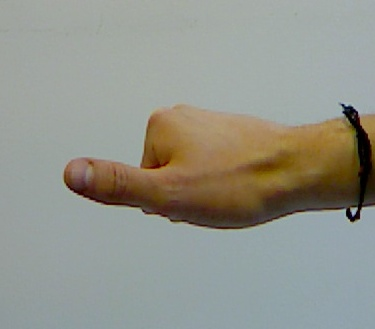
\includegraphics[width=0.2\linewidth]{figures/examples/6.jpg}
  \caption{\emph{fi1}, hand pose that yields poor classification performance}
  \label{fig:fi1}
\end{figure}


\begin{figure}[tb]
\centering{}
\subfloat[Sol]{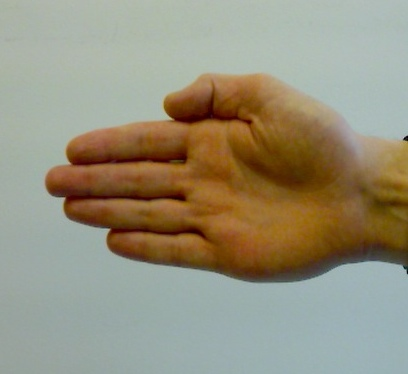
\includegraphics[width=0.2\linewidth,height=0.15\linewidth]{figures/examples/7.jpg}}
\hspace{0.03\linewidth}
\subfloat[Do]{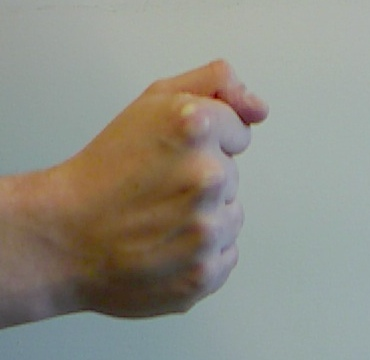
\includegraphics[width=0.2\linewidth,height=0.15\linewidth]{figures/examples/12.jpg}}
\hspace{0.03\linewidth}
\subfloat[Fa]{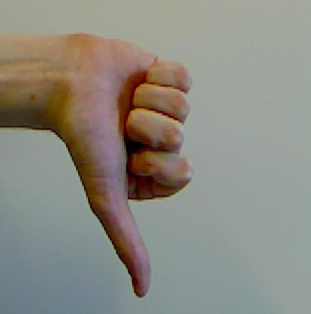
\includegraphics[width=0.2\linewidth,height=0.15\linewidth]{figures/examples/17.jpg}}
\hspace{0.03\linewidth}
\subfloat[Ti]{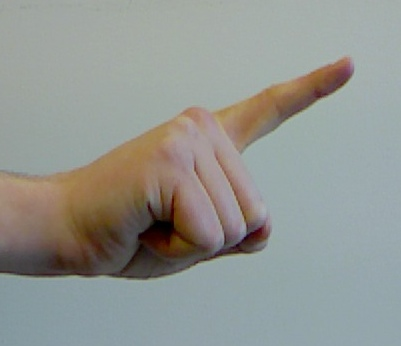
\includegraphics[width=0.2\linewidth,height=0.15\linewidth]{figures/examples/23.jpg}}
\hspace{0.03\linewidth}
\subfloat[Extra1]{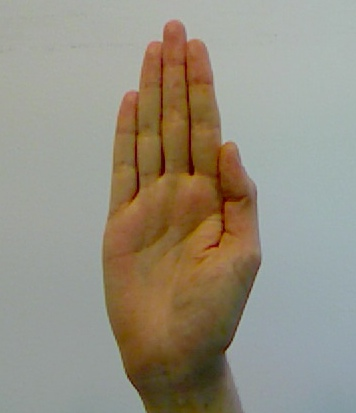
\includegraphics[width=0.2\linewidth,height=0.15\linewidth]{figures/examples/24.jpg}}
\hspace{0.03\linewidth}
\subfloat[Extra2]{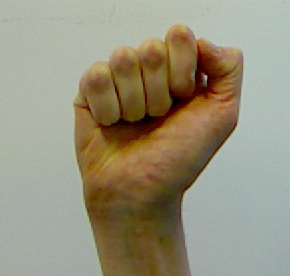
\includegraphics[width=0.2\linewidth,height=0.15\linewidth]{figures/examples/25.jpg}}
\hspace{0.03\linewidth}
\subfloat[Extra3]{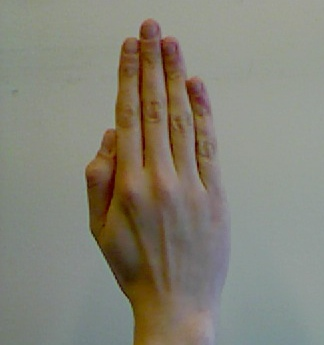
\includegraphics[width=0.2\linewidth,height=0.15\linewidth]{figures/examples/26.jpg}}
\caption{Hand poses that yield a high accuracy}
\label{fig:goodhands}
\end{figure}










\begin{table}
\centering
\begin{tabular}{llrr}
\hline\hline
Classifier 		& PCA		&  	Full scale	& Major scale	\\
\hline
KNN3 		&	no	&  	84.27\%		& 90.21\%		\\
KNN3	 	&	yes	& 	83.67\%		& 89.70\%		\\
SVM RBF ($c=1$ $\gamma=\frac{1}{|f|}$)	&	yes	& 	76.78\%	& 84.38\%	\\
SVM RBF ($c=2^6$ $\gamma=2^{-5}$)		&	no	&	86.02\%	& 90.88\% \\
SVM RBF ($c=2^6$ $\gamma=2^{-5}$)		&	yes	& 	86.85\% & \textbf{91.85\%} \\
SVM $\chi^2$ &	no	&	\textbf{87.92\%}		& 91.58\% \\
SVM $\chi^2$ &	yes	&	TODO		& TODO \\
\hline
\end{tabular}
\caption{k-fold per film using simple dataset only,}
\label{tab:perfilm}
\end{table}


\begin{table}
\centering
\begin{tabular}{lllrr}
\hline\hline
Dataset & Classifier & PCA	& Full scale	& Major scale \\
\hline
simple	& KNN3	&	no	& 72.93\%, & 82.63\% \\
simple	& SVM RBF ($c=2^6$ $\gamma=2^{-5}$) &	yes	& \textbf{79.71\%} & \textbf{86.70\%}	\\
\hline
full 	& KNN3 &	no	& 66.98\% & 76.32\%	\\
full 	& KNN3 &	yes	& 65.31\% & 76.00\%	\\
full 	& SVM RBF ($c=1$ $\gamma=\frac{1}{|f|}$) & yes	& 64.05\% & 74.42\%	\\
full 	& SVM RBF ($c=2^6$ $\gamma=2^{-5}$)	     & yes	& \textbf{73.38\%} & \textbf{81.44\%}	\\
full 	& SVM $\chi^2$ &	no	&  71.83\% &80.07\% \\
full 	& SVM $\chi^2$ &	yes	&  TODO & TODO \\
\hline
\end{tabular}
\caption{k-fold per person}
\label{tab:perperson}
\end{table}


\begin{table}
\centering
\begin{tabular}{lllcc}
\hline\hline
Descriptors & Classifier 		& pca		&  	Full scale	&	Major scale	\\
\hline
Hog & KNN3				& no	&	58.57\% 	&	72.78\%	\\
Hog & KNN3 				& yes	&	57.62\% 	&	72.17\%	\\
Hog & SVM RBF ($c=2^6$ $\gamma=2^{-5}$)			& yes & 62.14\%	&	73.39\%	\\
Hog & SVM RBF ($c=1$ $\gamma=\frac{1}{|f|}$)	& yes & 55.48\%	&	68.25\%	\\
Hog & SVM $\chi^2$ 		&	no	&	\textbf{63.81\%}		&	\textbf{74.71\%}	\\
Hog & SVM $\chi^2$		&	yes &	58.57\% 	&	71.98\% \\
\hline
SURF & KNN3				&	no	&	46.19\% 	&	60.17\%	\\
SURF & KNN3				&	yes &	44.05\%		& 56.65\% \\
SURF & SVM RBF ($c=2^6$ $\gamma=2^{-5}$)		& yes &	44.29\%	&	57.18\%	\\
SURF & SVM RBF ($c=1$ $\gamma=\frac{1}{|f|}$)	& yes &	40.00\%	&	53.28\%	\\
SURF & SVM $\chi^2$		&	no	&	37.93\%		&	47.91\%	\\
SURF & SVM $\chi^2$		&	yes	&	53.33\% 	&	65.13 \\
\hline
\end{tabular}
\caption{simple as trainset, complex as testset}
\label{tab:perset}
\end{table}


\begin{figure}[tb]
	\centering{}
	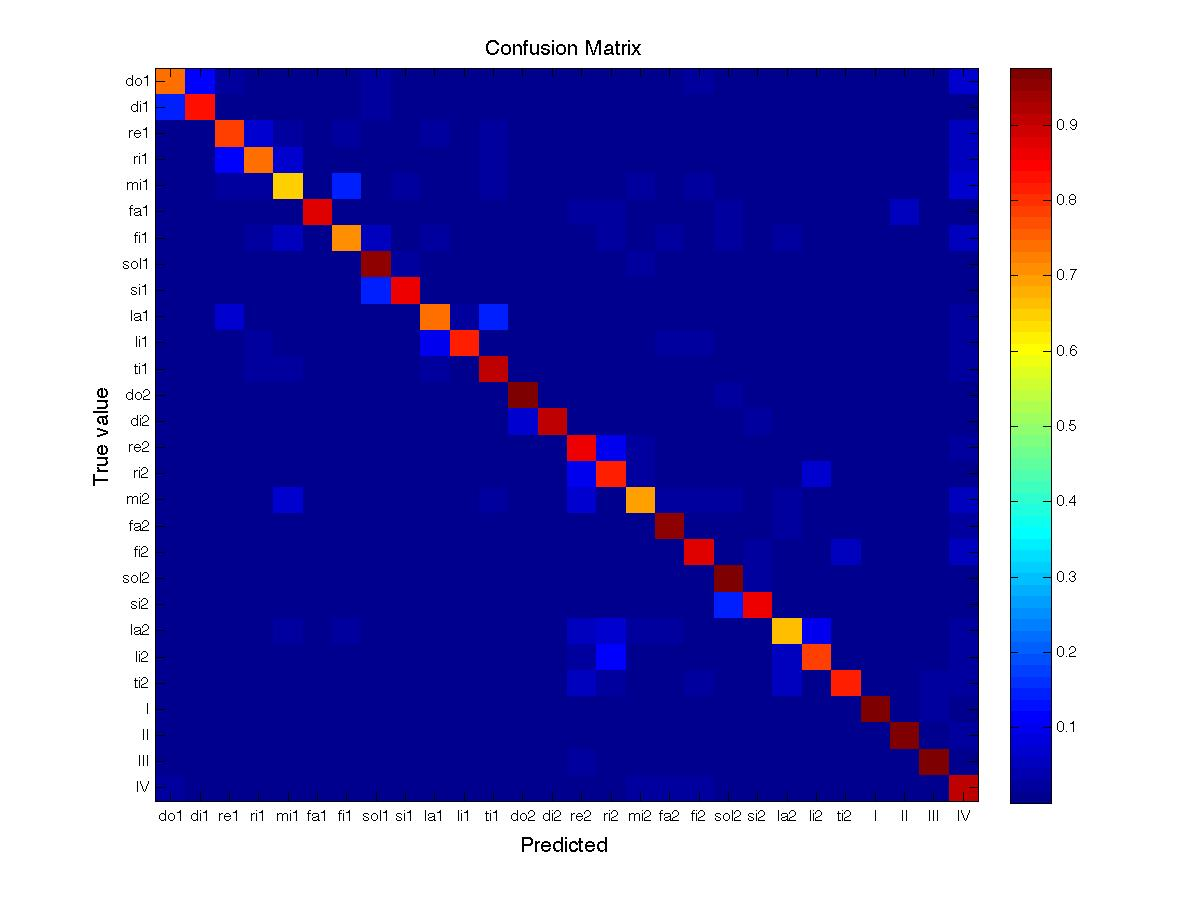
\includegraphics[width=\linewidth]{confmat/confusion.jpg}
	\caption{Confusion matrix using HOG, SVM $\chi^2$, n-fold, per film simple set}
	\label{fig:confusion}
\end{figure}




\subsection{Part II - Evaluating Sonic Gesture}

\subsubsection{Method}

\begin{figure}[tb]
\center{}
\subfloat[Without stabilizer]{
	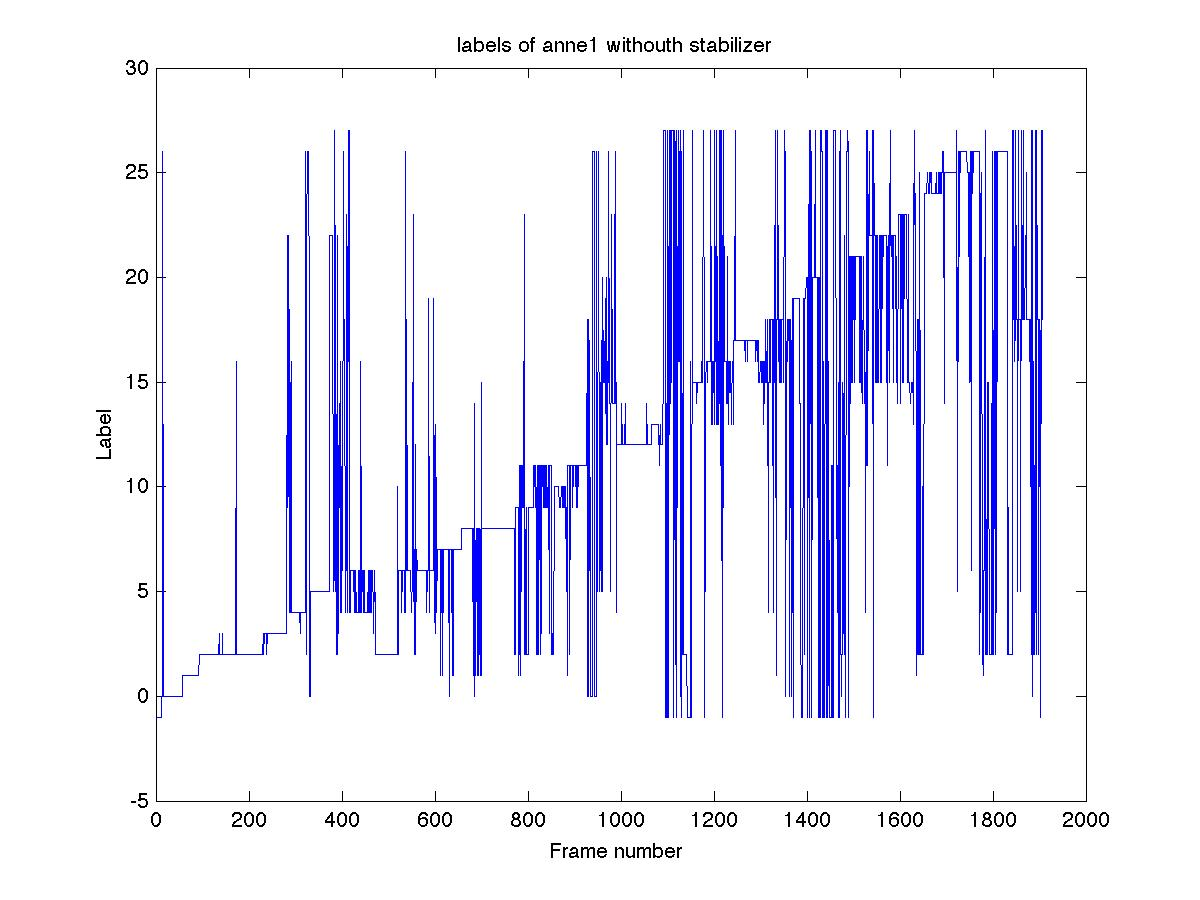
\includegraphics[width=0.3\linewidth]{figures/performance/anne1_unstable.jpg}}
\hspace{0.02\linewidth}
\subfloat[With stabilizer]{
	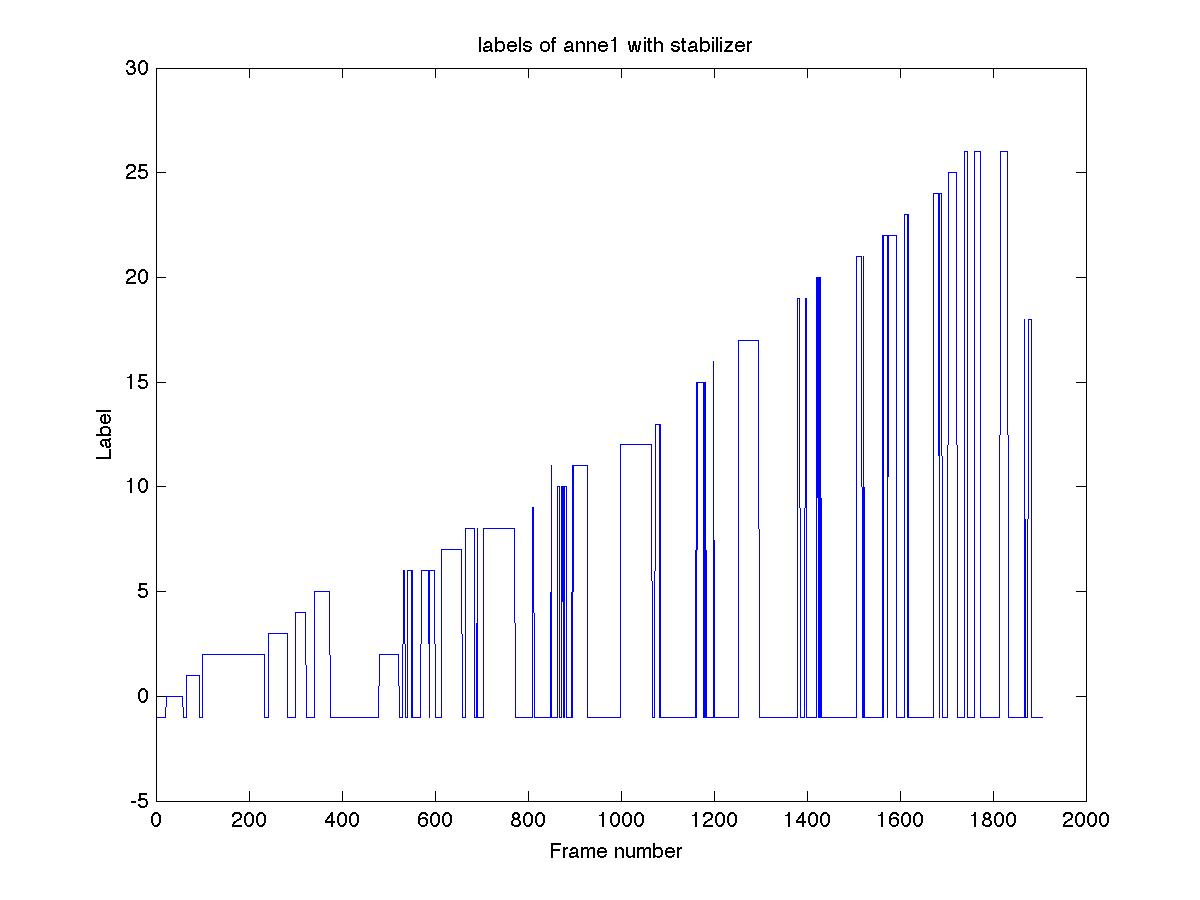
\includegraphics[width=0.3\linewidth]{figures/performance/anne1_stable.jpg}}
\hspace{0.02\linewidth}
\subfloat[Arbitrary movie with stabilizer]{
	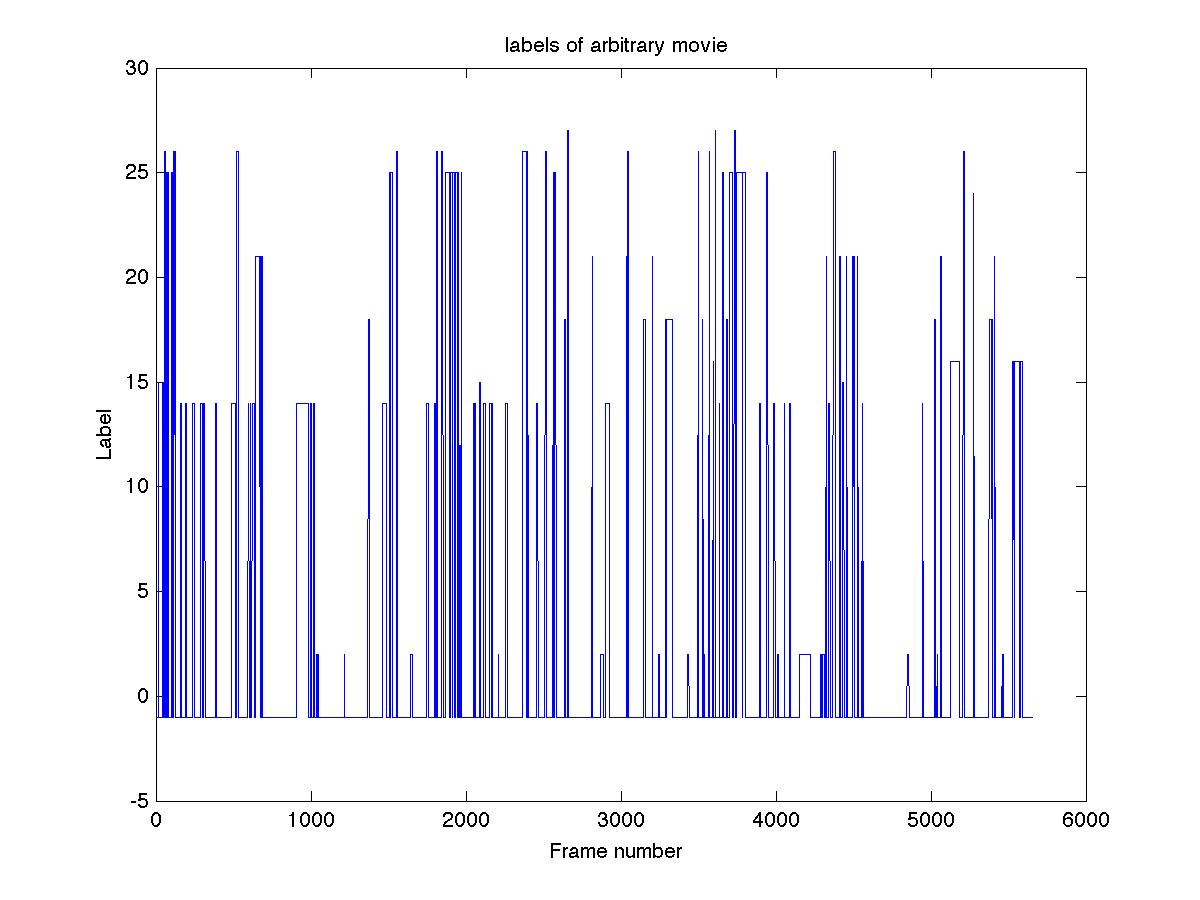
\includegraphics[width=0.3\linewidth]{figures/performance/heilige.jpg}}
\caption{Plots of labels per frame}
\label{fig:performances}
\end{figure}

To evaluate Sonic Gesture in the time domain, the sequential output must be evaluated. Sonic gesture outputs for every frame the estimated label for each hand. Constructing a ground truth for each frame is a difficult, time consuming and subjective process. The material is also `polluted' with wrong hand poses caused by misunderstanding or misinterpretation. In some cases there are also more people in the image than only the test subject. To evade these problems a different evaluation method is used, where the consecutive changes in labels is evaluated. Since the goal for each recorded movie in the dataset was to record a person performing the 28 hand poses sequentially, the ground truth is a ordered list of all labels.

\autoref{fig:performances} visualized the sequence of labels in three cases, (a) when no stabilizer is used, a erratic pattern is the result. When the stabilizer is used (b) a more smooth incremental label pattern is visible. (c) shows the label sequence of an arbitrary movie. Scoring these patterns would be useful for comparison an tweaking. This can be done by calculating the Damerau-Levenshtein distance to the ground truth.

the output of Sonic Gesture for all movies is stored. This results in a long list of labels - one label for each frame - for each move. In each list all repeating labels are replaced with one instance of that label. This reduces the length of each list significantly. Now this list can be used to compute the Damerau-Levenshtein Distance.

The Damerau-Levenshtein Distance algorithm is shown in Algorithm~\autoref{alg:dameraulevenshtein}. The algorithm calculated to number of deletions, insertions, substitutions and transpositions required to transform one string into an other. The maximum number of operations is equal to the length of the shortest string. Because of the ground truth's length of 28 the minimum will always be 28 or less. This way the distance can be safely normalized and divided by 28, so all distances can be easily compared.

\begin{algorithm}
\caption{DamerauLevenshteinDistance(str1, str2)}
\label{alg:dameraulevenshtein}
\begin{algorithmic}
   \REQUIRE a string str1
   \REQUIRE a string str2
   \ENSURE The distance between str1 and str2

   \medskip

   \FOR{$i = 1$ to lenStr1}
       \STATE $\mathbf{D}[i, 0] \Leftarrow i$
   \ENDFOR
   \FOR{$j = 1$ to lenStr2}
       \STATE $\mathbf{D}[0, j] \Leftarrow j$
   \ENDFOR
   \FOR{$i = 1$ to lenStr1}
       \FOR{$j = 1$ to lenStr2}
       		\IF{str1$_{i} =$ str2$_{j}$}
				\STATE cost $\Leftarrow 0$
            \ELSE
				\STATE cost $\Leftarrow 1$
			\ENDIF
			\STATE $x \leftarrow \mathbf{D}_{i-1, j  } + 1$ % deletion
			\STATE $y \leftarrow \mathbf{D}_{i  , j-1} + 1$ % insertion
            \STATE $z \leftarrow \mathbf{D}_{i-1, j-1} + $ cost % substitution
            \STATE $\mathbf{D}_{i, j} \Leftarrow \min(x, y, z)$
            \IF {(str1$_{i} =$ str2$_{j-1}$) $\wedge$ (str1$_{i-1} =$ str2$_{j}$)}
				\STATE $\mathbf{D}_{i, j} \Leftarrow \min(
                	\mathbf{D}_{i, j},
                    \mathbf{D}_{i-2, j-2} + $ cost  % transposition
                )
			\ENDIF
		\ENDFOR
	\ENDFOR
   \RETURN $\mathbf{D}_{lenStr1, lenStr2}$

\end{algorithmic}
\end{algorithm}
	
\subsubsection{Results}
\autoref{tab:distance} contains all distances, grouped per dataset. The numbers in table heading are the movie number of that column. The average column is the \textit{average} of all movies per person. The average per person column lists the same distances, but without using the stabilizer discussed in \autoref{subsec:stabilizer}. As you see this has a dramatic impact on the performance. The average distance for the simple set is 0.27, for the complex set 0.35. 



\begin{table}
\centering
\begin{tabular}{p{0.4in}rrrrrrrp{0.55in}}
\hline
Dataset & Name	& 1 & 2 & 3 & 4 & 5 & Average & Average without stabilizer\\
\hline
Simple & Anne	&	0.43	&	0.32	&	0.25	&	0.29	&	0.14	&	0.28	&	0.88 \\
 & Arjan	&	0.46	&	0.25	&	0.25	&	0.07	&	0.29	&	0.26	&	0.83 \\
 & Gijs	&	0.14	&	0.18	&	0.21	&	0.21	&	0.14	&	0.18	&	0.87 \\
 & Ivo	&	0.07	&	0.11	&	0.07	&	0.11	&	0.04	&	0.08	&	0.86 \\
 & Jasper 1	&	0.68	&	0.46	&	0.21	&	0.21	&	0.43	&	0.40	&	0.85 \\
 & Peter	&	0.25	&	0.29	&	0.25	&	0.32	&	0.18	&	0.26	&	0.86 \\
 & Hanne	&	0.32	&	0.00	&	0.04	&	0.25	&	0.07	&	0.14	&	0.91 \\
 & Jasper 2	&	0.32	&	0.18	&	0.18	&	 	&	 	&	0.23	&	0.90 \\
 & Ork	&	0.21	&	0.18	&	0.14	&	 	&	 	&	0.18	&	0.86 \\
 & Roberto	&	0.68	&	0.29	&	0.46	&	 	&	 	&	0.47	&	0.83 \\
 & Xirong	&	0.61	&	0.50	&	0.36	&	 	&	 	&	0.49	&	0.88 \\
\hline
Complex & Gosia	&	0.57	&	0.32	&	0.21	&	 	&	 	&	0.37	&	0.88 \\
 & Hamdi	&	0.50	&	0.43	&	0.54	&	 	&	 	&	0.49	&	0.87 \\
 & Michael	&	0.21	&	0.29	&	0.46	&	 	&	 	&	0.32	&	0.90 \\
 & Sil	&	0.50	&	0.61	&	0.46	&	 	&	 	&	0.52	&	0.83 \\
 & Victoria	&	0.32	&	0.21	&	0.18	&	 	&	 	&	0.24	&	0.88 \\
 & Chu	&	0.29	&	0.21	&	0.07	&	 	&	 	&	0.19	&	0.89 \\
\hline
Complex & Koen	&	0.39	&	0.32	&	0.39	&	 	&	 	&	0.38	&	0.88\\
with & Bas	&	0.54	&	0.43	&	0.32	&	 	&	 	&	0.44	&	0.90 \\
poster & Stratis	&	0.43	&	0.11	&	0.18	&	 	&	 	&	0.24	&	0.86 \\


\hline
\end{tabular}
\caption{Damerau-Levenshtein distance of all movies}
\label{tab:distance}
\end{table}



\subsection{Part III - The Search for Spock}

\subsubsection{Method}
To show that Sonic Gesture can also work with non artificial video material a third experiment was constructed. For this experiment a collection of real fragments of movies and pictures of people performing the `Vulcan Salute' was gathered. The Vulcan Salute is greeting hand gesture and was popularised by the half-Vulcan character Mr. Spock on the Star Trek television series in end of the 1960s. \autoref{fig:spock} is a movie fragment of Mr. Spock giving the hand salute. The original dataset used for the previous experiments was extended with a 29th hand pose, the vulcan salute. 

\begin{figure}[tb]
\centering{}
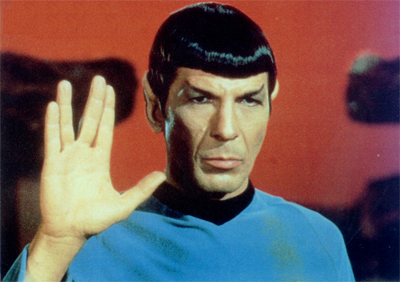
\includegraphics[width=0.6\linewidth]{figures/spock/salute.png}
\caption{Mr. Spock giving the Vulcan Salute}
\label{fig:spock}
\end{figure}


\subsubsection{Results}
\autoref{fig:vulcangood} shows eight examples of successful classification of the vulcan salute. The images are cutout screenshots of the implementation of Sonic Gesture. The upper left window is the input, the upper right window is the segmented and labeled visualisation. A green square indicates a right hand and yellow left. The bottom squares show the estimated hand poses, the left square for the left hand and the right square for the right hand. For the visualisation of the detected Vulcan Salute the picture of Mr. Spock is used.

\autoref{fig:vulcanfail} shows two screenshots of failed segmentation. Sonic Gesture fails on the first salute - performed by Condolisa Rise - because the skin segmentation fails. The skin colour of her face has more in common with the wall than with her hand. The second failure case is performed by Simon Pegg, here the segmentation is correct, but classification is just wrong. More training data could fix this problem.

\begin{figure}[tb]
\centering
\subfloat{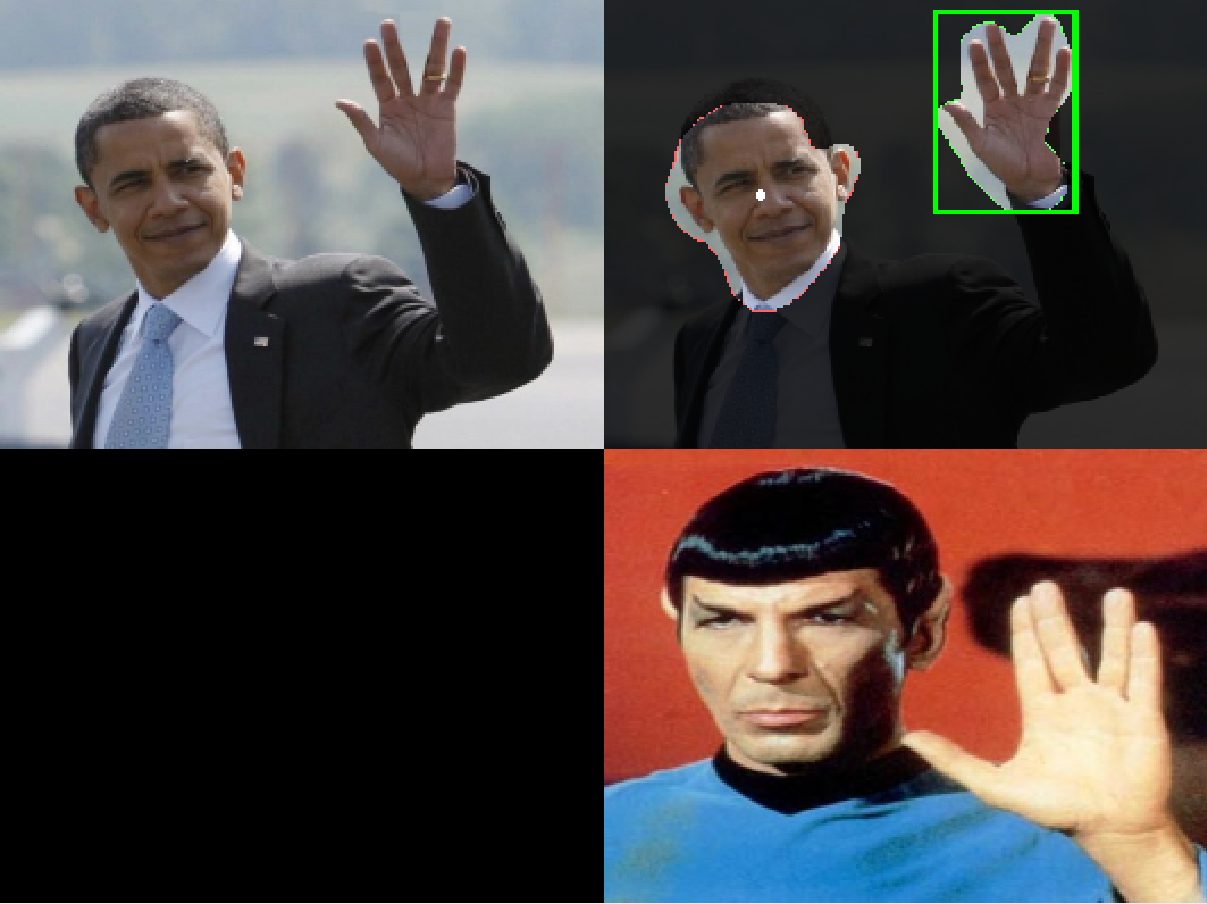
\includegraphics[width=0.3\linewidth,height=0.25\linewidth]{figures/spock/good1.png}}
\hspace{0.2\linewidth}
\subfloat{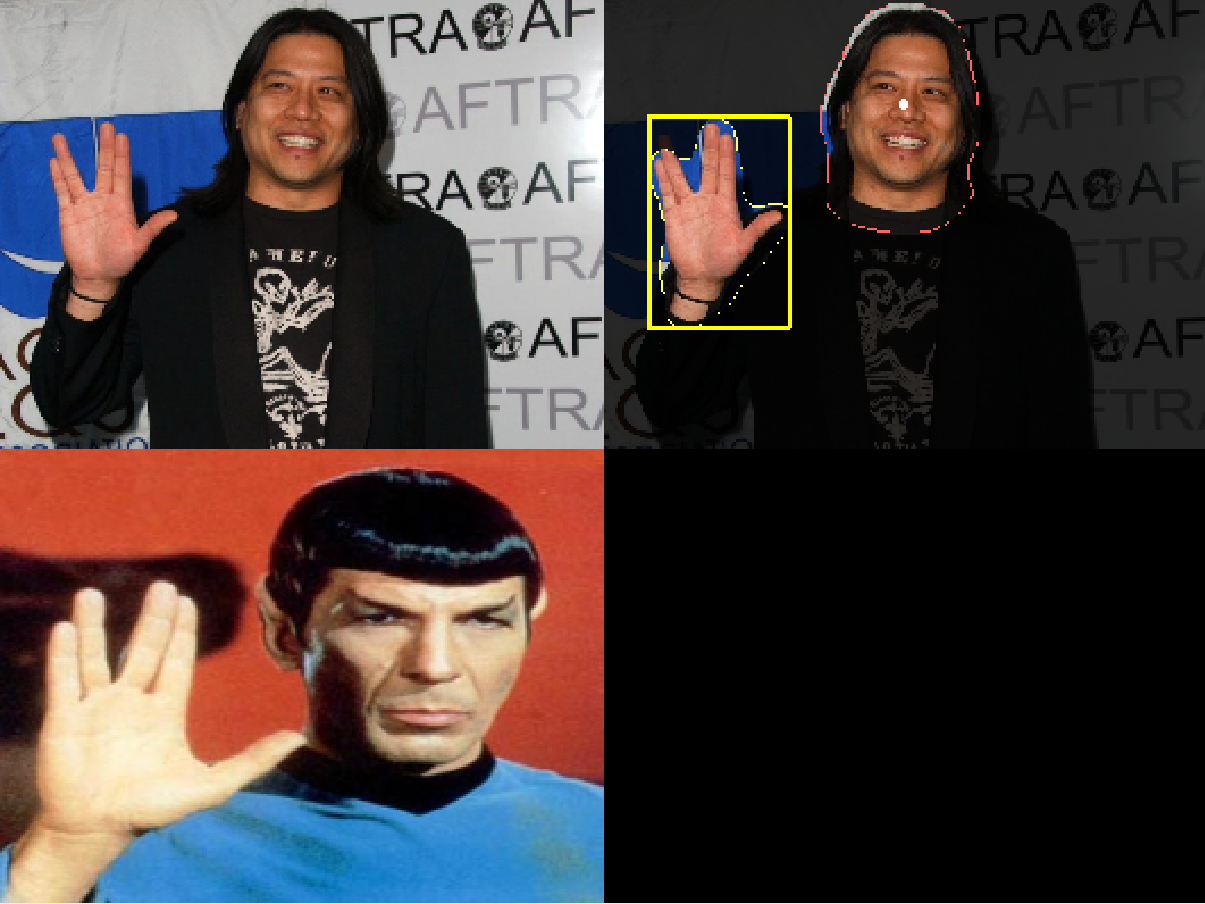
\includegraphics[width=0.3\linewidth,height=0.25\linewidth]{figures/spock/good2.png}}
\hspace{0.2\linewidth}
\subfloat{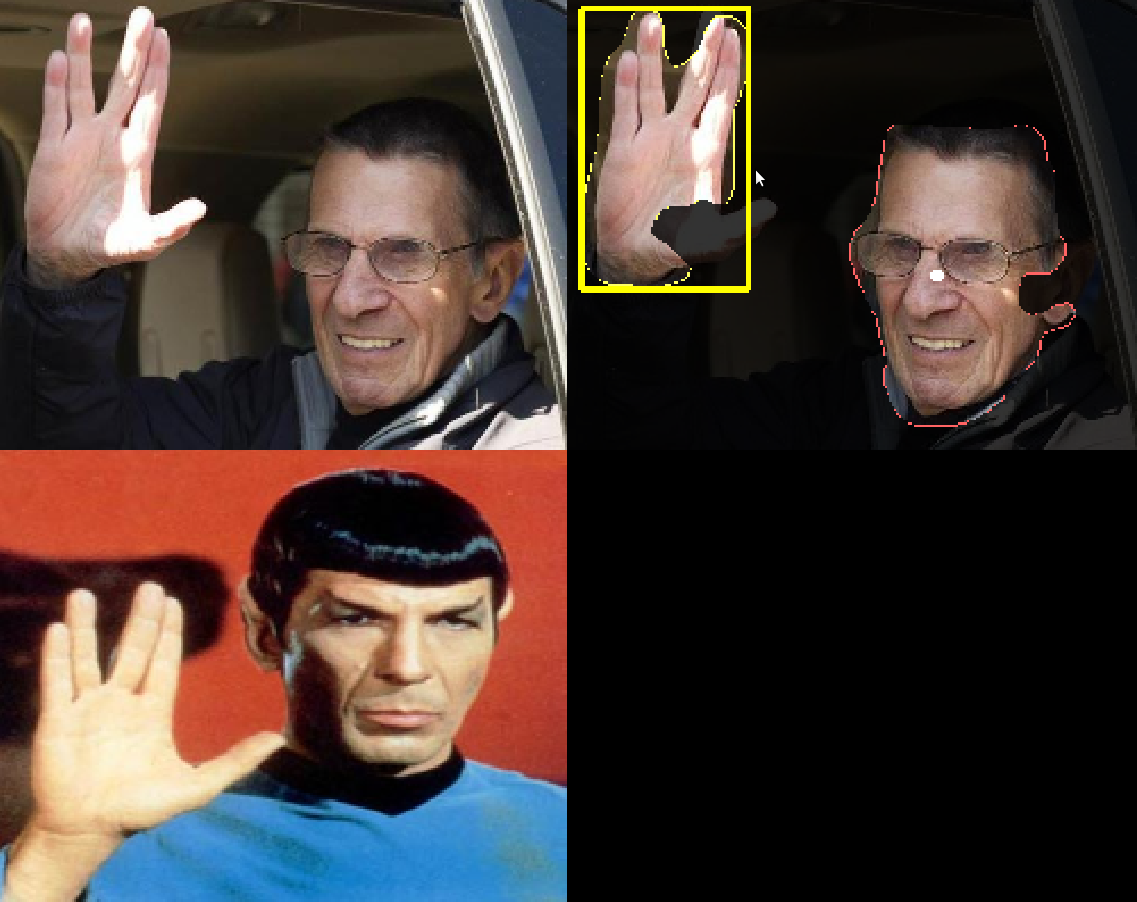
\includegraphics[width=0.3\linewidth,height=0.25\linewidth]{figures/spock/good3.png}}
\hspace{0.2\linewidth}
\subfloat{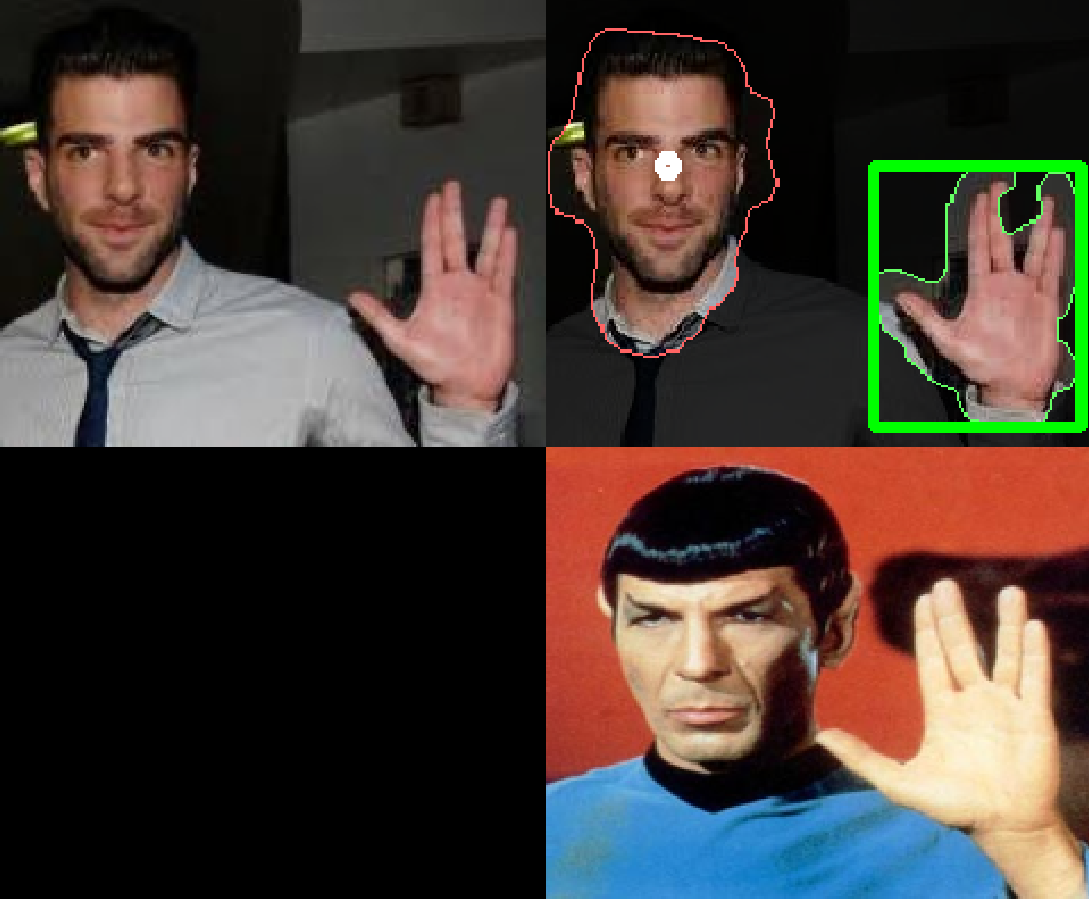
\includegraphics[width=0.3\linewidth,height=0.25\linewidth]{figures/spock/good4.png}}
\hspace{0.2\linewidth}
\subfloat{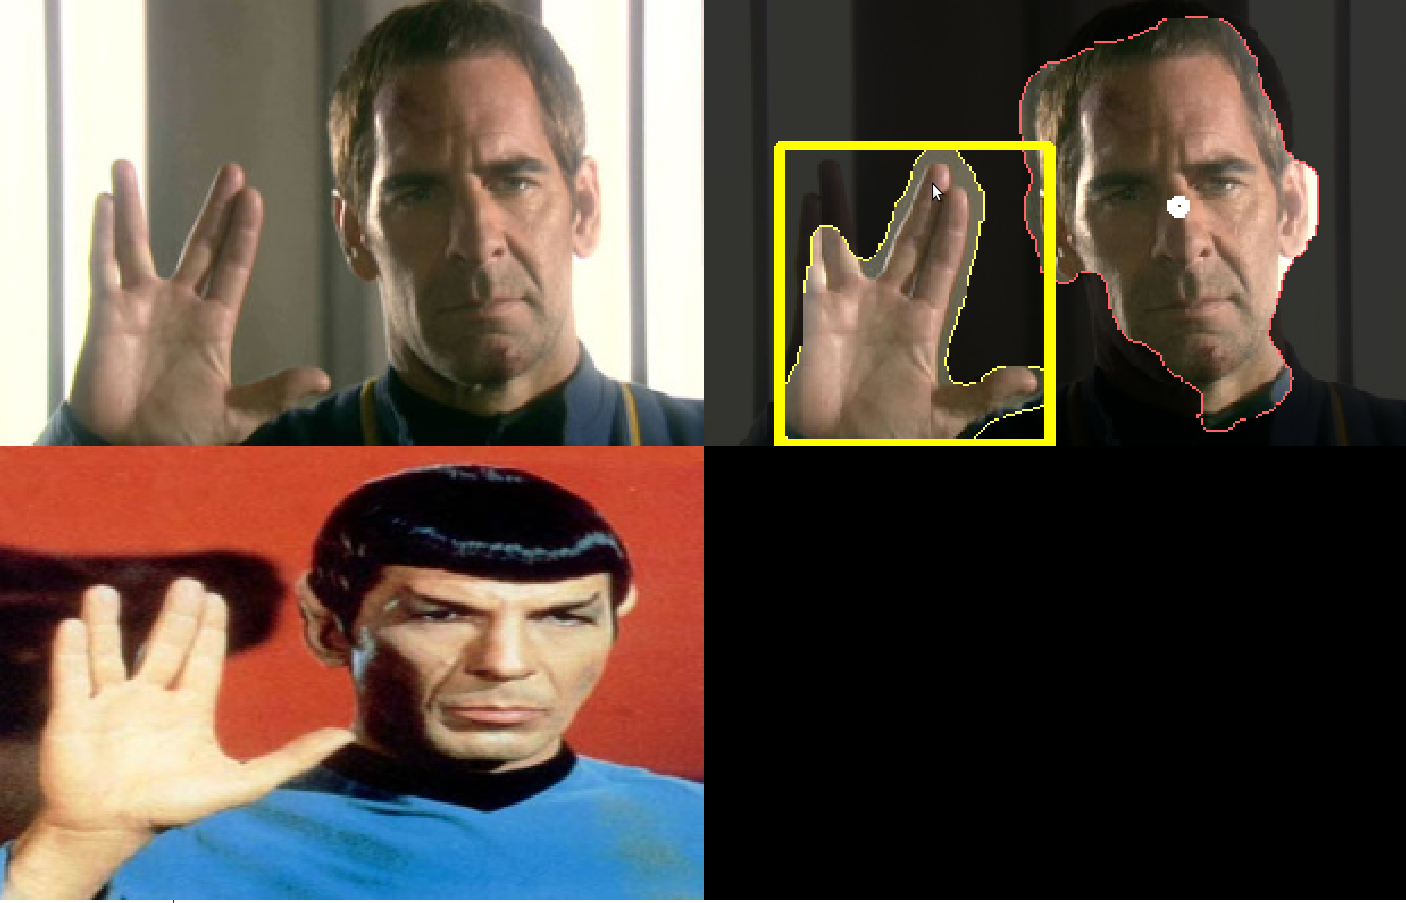
\includegraphics[width=0.3\linewidth,height=0.25\linewidth]{figures/spock/good5.png}}
\hspace{0.2\linewidth}
\subfloat{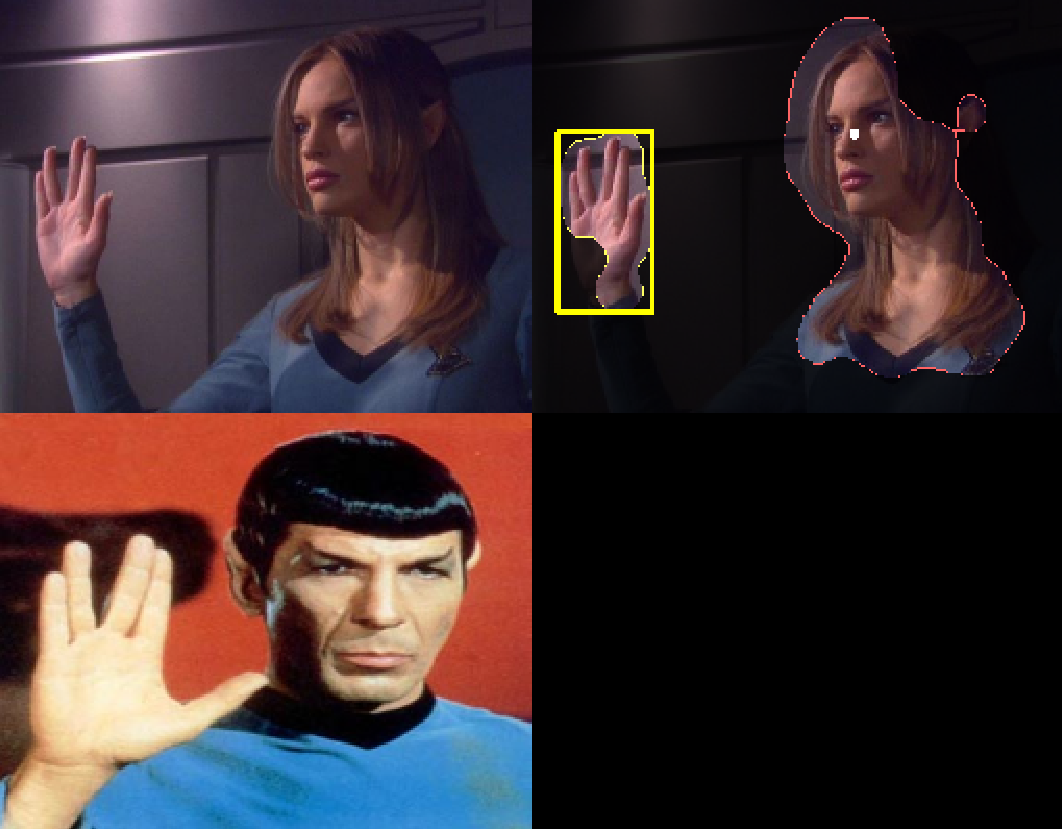
\includegraphics[width=0.3\linewidth,height=0.25\linewidth]{figures/spock/good6.png}}
\hspace{0.2\linewidth}
\subfloat{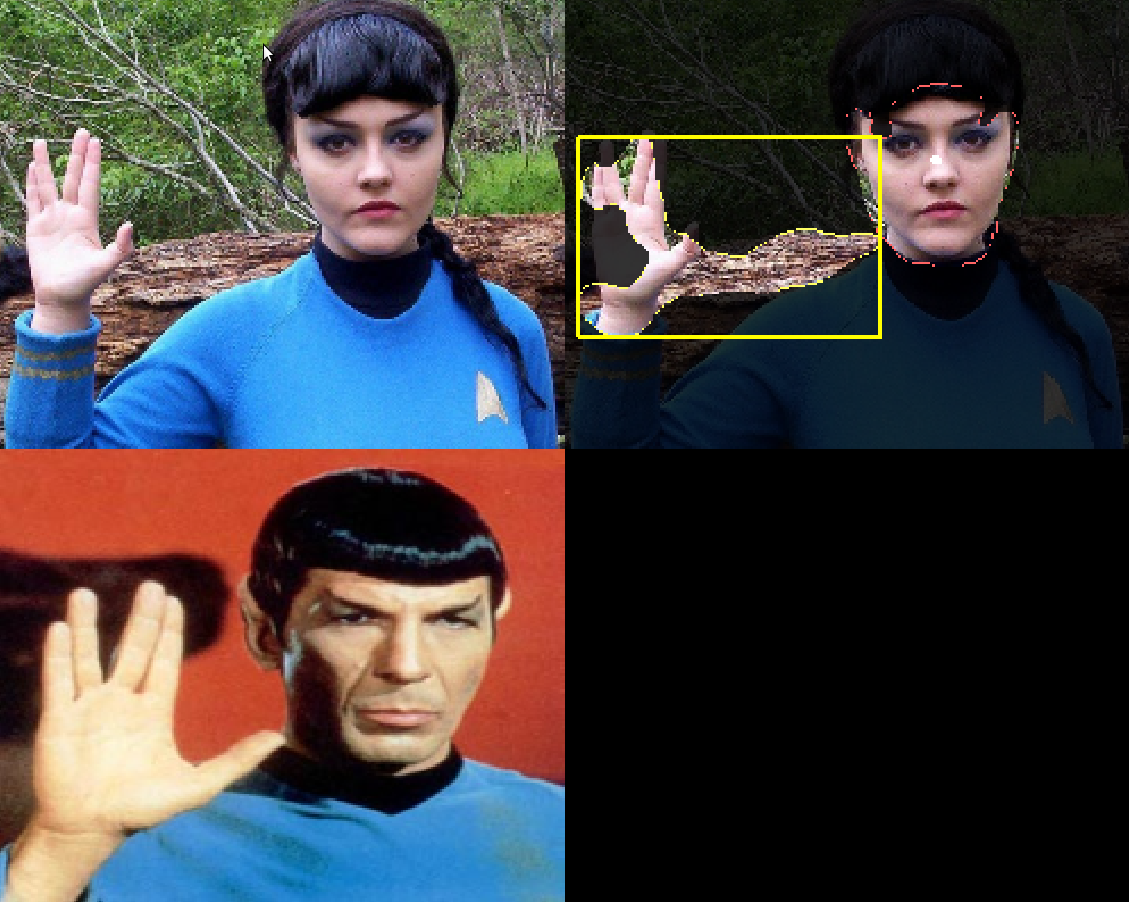
\includegraphics[width=0.3\linewidth,height=0.25\linewidth]{figures/spock/good7.png}}
\hspace{0.2\linewidth}
\subfloat{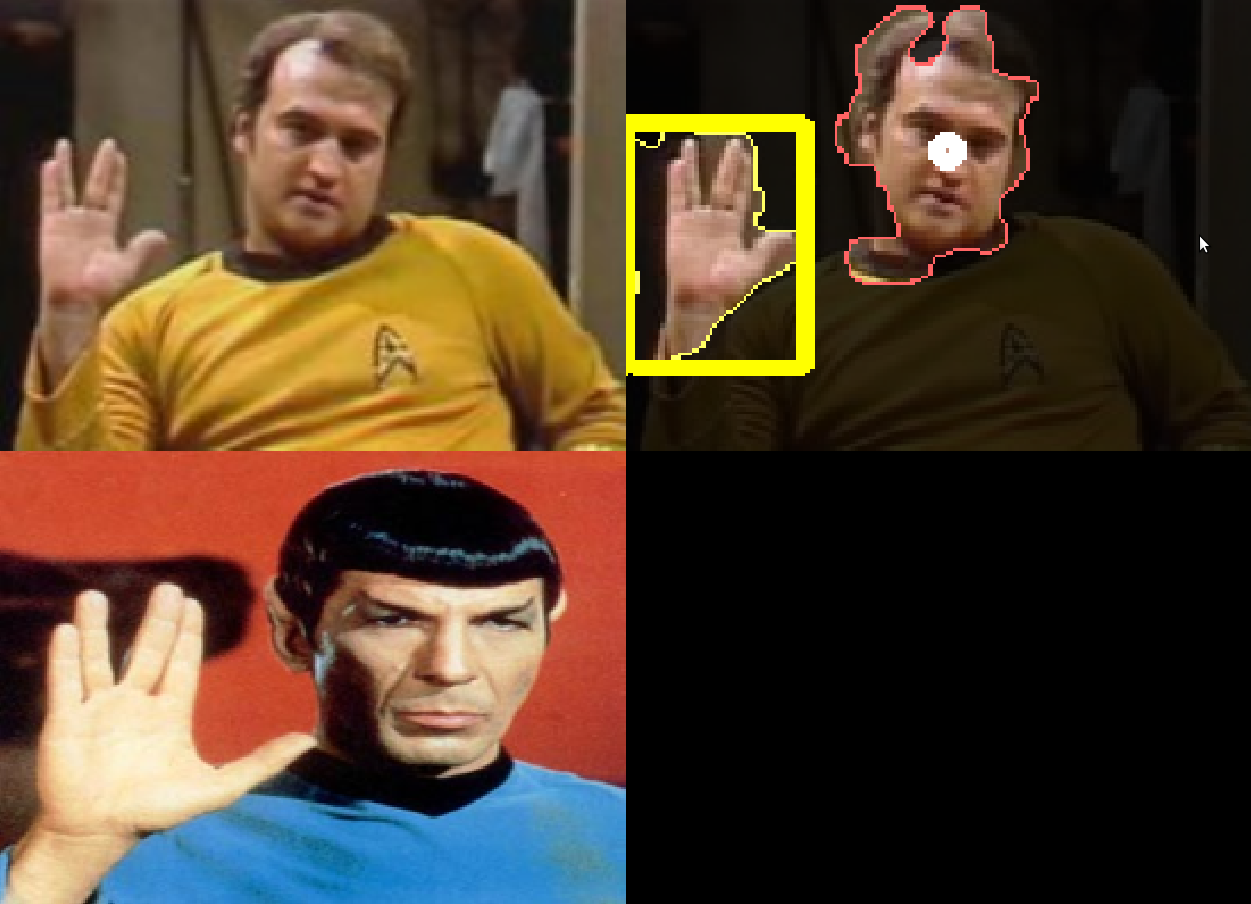
\includegraphics[width=0.3\linewidth,height=0.25\linewidth]{figures/spock/good8.png}}
\hspace{0.2\linewidth}
\caption{Successful detection of Vulcan salute}
\label{fig:vulcangood}
\end{figure}


\begin{figure}[tb]
\centering
\subfloat{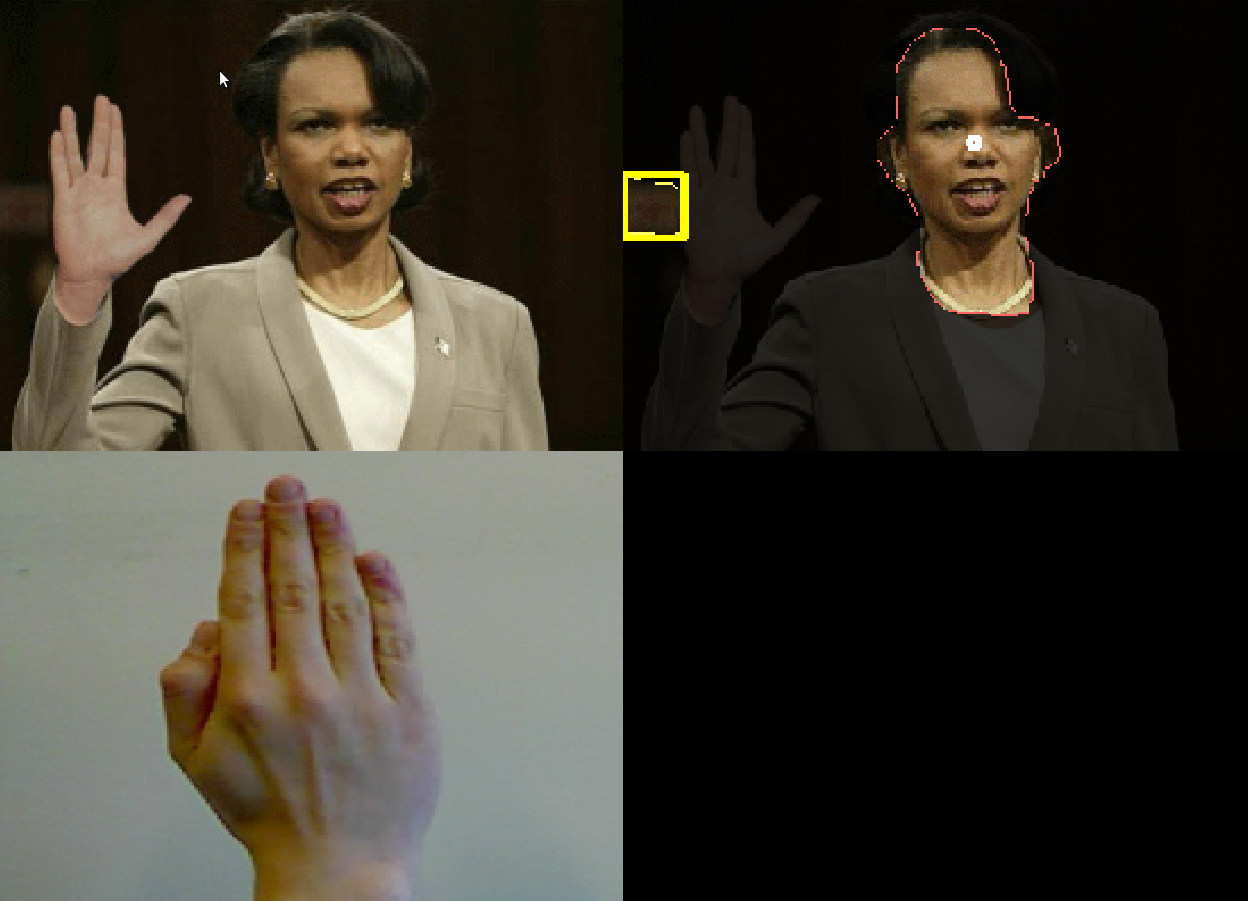
\includegraphics[width=0.3\linewidth,height=0.25\linewidth]{figures/spock/fail1.png}}
\hspace{0.2\linewidth}
\subfloat{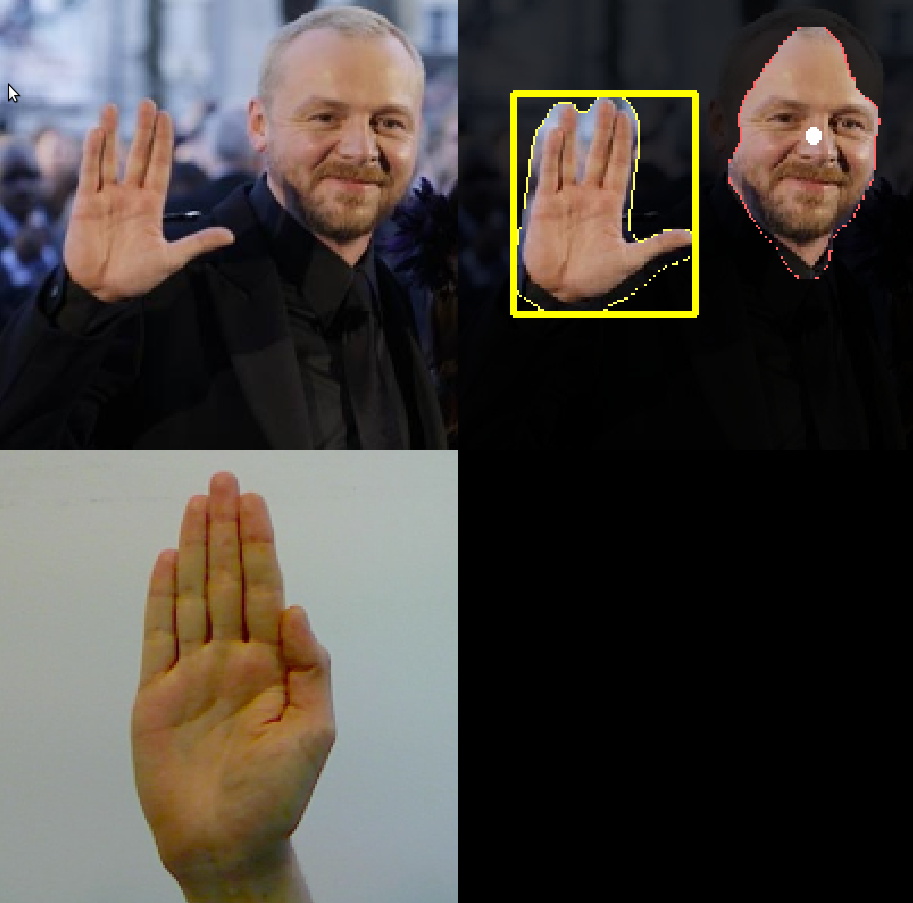
\includegraphics[width=0.3\linewidth,height=0.25\linewidth]{figures/spock/fail2.png}}
\caption{Failed detection of Vulcan salute}
\label{fig:vulcanfail}
\end{figure}


